\documentclass[11pt,a4paper]{report}

\usepackage[top=1.5in,bottom=1.5in,left=1in,right=1in]{geometry}
\usepackage{pdflscape}
\usepackage{enumitem}
\usepackage{graphicx}
\usepackage[nottoc]{tocbibind}
\usepackage[square,comma,numbers]{natbib}
\usepackage{listings}
\usepackage{color}
\usepackage{float}
\usepackage[parfill]{parskip}

\graphicspath{ {./images/} }

\definecolor{javared}{rgb}{0.5,0,0.33} % for keywords
\definecolor{javablue}{rgb}{0.16,0,1} % for strings
\definecolor{javagreen}{rgb}{0.25,0.5,0.37} % comments
\definecolor{javadocblue}{rgb}{0.5,0.62,0.75} % javadoc

\renewcommand{\labelitemi}{$-$}
\renewcommand{\labelitemii}{$\bullet$}
\renewcommand{\labelitemiii}{$\diamond$}

\lstset{language=Java,
basicstyle=\ttfamily,
keywordstyle=\color{javared}\bfseries,
stringstyle=\color{javablue},
commentstyle=\color{javagreen},
morecomment=[s][\color{javadocblue}]{/**}{*/},
numbers=left,
numberstyle=\tiny\color{black},
stepnumber=2,
numbersep=10pt,
tabsize=4,
showspaces=false,
showstringspaces=false,
breaklines=true,
}

\bibliographystyle{IEEEtranS}

\begin{document}
\title{{\normalsize G52GRP Final Report}\\EduCraft\\\textit{Minecraft as a Collaborative Learning Tool}}
\author{Group \texttt{gp13-pxb1}:\\
            Tosin Afolabi (\texttt{ooa02u})\\
            Janos Bana (\texttt{jxb12u})\\
            Eze Benson (\texttt{exb02u})\\
            Alastair Kerr (\texttt{axk02u})\\
            Ian Knight (\texttt{iak12u})\\
            Ying Wang (\texttt{yxw03u})
            }
\maketitle

\tableofcontents

\chapter{Introduction and Background}
\label{ch:introduction}
The EduCraft project is concerned with developing a series of
extensions\footnote{These are commonly called `mods'. Throughout the report,
we will refer to our product as `the mod'.} for the popular computer game
Minecraft, aimed at promoting collaborative learning in primary schools,
particularly with reference to numeracy education. In this first section, some
of the advantages of collaborative learning are explored in contrast to
conventional teaching methods, and the game of Minecraft is introduced in the
context of education.

\section{Collaborative learning}
\begin{quote}
``Group interaction allows students to negotiate meanings, to express
themselves in the language of the subject and to establish a more intimate
and dialectical contact with academic and teaching staff than formal
methods permit.'' \cite[p.~1]{jacques00}
\end{quote}
Group work has long been recognised as a key component in any form of
successful education---it enables students to become more involved in their
own work, and to engage with it in a different manner from what is normally
seen in classrooms. Johnson and Johnson observe that ``The human species seems
to have a \textit{cooperation imperative}'', and that cooperation plays
a central role in most areas of life \cite[p.~12]{johnson94}.

Collaborative or cooperative learning is contrasted with two other `goal
structures': competitive learning, and individualistic learning. Competitive
learning consists of activities which set the students tasks which some
are expected to `win', by getting the highest score or completing the activity
in the shortest time, for example. Individualistic learning is learning where
there is no interaction between students at all---no comparisons are made,
and students are solely concerned with working by themselves.

Johnson and Johnson argue that each of these goal structures has a role
to play in education, but that each is suitable for different
purposes \cite{johnson94}.  Collaborative learning, specifically, is to
be used in situations where the material being taught is especially
complex or conceptual. This makes it ideal for use in maths lessons:
Yackel, \textit{et al.} describe the benefits of group work in teaching maths
to second-grade\footnote{Roughly equivalent to year 5 (ages 7--8) in the UK}
students in the US \cite{yackel91}.

\section{Minecraft}
\begin{quote}
``Minecraft is a game about breaking and placing blocks. At first, people
built structures to protect against nocturnal monsters, but as the game grew
players worked together to create wonderful, imaginative things.''
\cite{website:minecraft}
\end{quote}

Minecraft was initially developed in 2009, as a game where players could
explore a randomly-generated world and place blocks to build structures. From
the outset, Minecraft was not designed as a game that could be `won'---in
game industry terms, it was intended to be a `sandbox' game where players set
their own goals.

There have been a number of articles written exploring the potential use of
Minecraft in supporting education \cite{brand13}, \cite{short12}. Habgood has
already established the usefulness of computer games in general in education
\cite{habgood07}; the question is whether Minecraft can be used in the ways
that he suggests. This is what EduCraft seeks to establish, at least tentatively.

The official Minecraft Wiki has its own page dedicated to describing possible ways
of using Minecraft in education \cite{website:mcwiki}, and suggests using the
game's in-built system of building items:
\begin{quote}
    ``The crafting system can help in teaching basic math (e.g. I need 3 Sugar
    Cane for Paper), which transitions to multiplication (I need 3 Paper and 1
    Leather for a Book, and 3 Books for a Bookshelf, so I need 9 Paper and 3 Leather
    all together) and division (When I create Paper I get 3 at once, so 9/3 =
    3 times per Bookshelf I'll have to create Paper).''
\end{quote}

We intend to build something more overtly mathematical than this basic concept,
and the remainder of the report describes the requirements that have been set
for the project, along with a record of our initial design and prototypes.

\chapter{Requirements Specification}

\section{Functional requirements}
\begin{enumerate}

	\item The game must cater for users who are currently at level 2 of Key Stage 2 mathematics.
	\begin{enumerate}[label={1.\arabic*},nolistsep,leftmargin=*]
		\item There must be a puzzle in the game which challenges the users knowledge of subtraction facts up to 10.
		\item There must be a puzzle in the game which challenges the users knowledge of number ordering from 0 - 100.
		\item There must be a puzzle in the game which challenges the users knowledge of number sequencing. This must include odd and even numbers.
	\end{enumerate}

	\item The game must cater for users who are currently at level 3 of Key Stage 2 mathematics.
	\begin{enumerate}[label={2.\arabic*},nolistsep,leftmargin=*]
		\item There must be a puzzle in the game which challenges the users knowledge of the 2,3,4,5 and 10 times table.
		\item There must be a puzzle which forces a user to use multiplication or division to solve it. The multiplication or division must only be used with whole numbers. When choosing numbers for division numbers with remainders are to be included.	
		\item The game should include puzzles which involves breaking entities into simple fractions.
		\item Within the game there should be puzzles which require users to equate simple fractions.
	\end{enumerate}
	
		\item The game must cater for users who are currently at level 4 of Key Stage 2 mathematics.
		\begin{enumerate}[label={3.\arabic*},nolistsep,leftmargin=*]
			\item Puzzles must exist within the game which can only be solved using division by 10 or 100. The entities being divided must be whole numbers.
			\item A puzzle must exist which tests users upon their knowledge of multiplication facts up to 10x10. This puzzle should then go on to test whether the user can quickly derive correct division facts.
			\item Within the game there should be a puzzle which involves adding and subtracting entities which represent decimal numbers to 2 decimal places.
			\item A puzzle should exist which forces the user to order decimal numbers. These decimal numbers can be up to three decimal places in length.
		\end{enumerate}
		
	\item Levels in the game must be constructed in such a way that each user contributes to a problem before all the users can progress. A user must contribute within the game physically.
	\item The game must not be single player and should allow players in groups of 3-4 to play together.
	\item The players should be able connect to dedicated servers to play the game.
	
	\item The mod must implement coins as one of the visual representations of numbers.
	
	\item The mod must have custom weapons which can be used to defeat zombies.
	
	\item Coins and other visual representations of numbers must be collected by defeating zombies.
	
	\item Zombies must not drop numbers or coins if the user does not defeat them using the specific mathematical weapon.
	
	\item Zombies must have a number above their head clearly visible to the player indicating what number they drop upon being defeated.
	
	\item Zombies should drop a number or coins equal to the number stated above the zombie's head.
	
	\item Players must be able to craft all mathematical operators using items collected throughout the level. (Mathematical operators being +,-,*,/) 
	
	\item Each mathematical operator must be represented visually in a way which is commonly understood by people of the specified age group.
	
	\item Puzzles must be solved in chambers as well as open world spaces.
	
	\item Players should not be allowed to progress until the puzzle they are currently on is completed.
	
	\item Mathematical operators must be usable objects and not weapons.
	
	\item Mathematical operators will be crafted using items which have been ascertained through resource collecting, where resource collecting is the action of getting items in any way but defeating zombies.
	
	\item Equations must be able to be crafted using mathematical operators and numbers collected from defeated zombies.
		
\end{enumerate}

\section{Non-functional requirements}
\begin{enumerate}
	\item The game must be implemented in Minecraft through a mod.
	\item The mod should work on Minecraft version 1.6.4.
	\item The mod must work on the windows operating system.
	\item The mod must work on a machine which has the minimum requirements of Minecraft or better.
	\item The game should abide by the ethics code in place within the education system for those between the ages of 8 and 11.
\end{enumerate}


\chapter{Design}
\label{ch:design}
% report goes here

\section{Educational Design Decisions}

\section{Game Design}
The aim of our game design was to efficiently encode collaborative learning in the mechanics of the game. This section will list and describe all the additional elements that we decided to add to the existing Minecraft 1.6.4 core game in order to create a playable mod that would fulfill our requirements. We gradually introduced new elements as and when required.
\newline\newline
The mod is set to be played in adventure mode\footnote{Adventure mode is a game mode intended for player-created maps by limiting some of the gameplay in Minecraft, in which the player cannot directly destroy most blocks to avoid spoiling adventure maps or griefing servers. Most blocks cannot be destroyed without the proper tools. However, players can still interact with mobs and craft items.\cite{website:minecraft-adventure}}.
We have tried to preserve as much of the Minecraft concepts in our extension as possible, so that players familiar with the game can easily understand the mechanics of our mod. Inexperienced users will also get to know the Minecraft philosophy whilst using our extension and will be able to play the original game or some other mods without any problems in the future.

\begin{itemize}
\item \huge Items\large \footnote{Items are objects which only exist within the player's inventory and hands - which means, they cannot be placed in the game world. Some items simply place blocks or entities into the game world when used. They are thus an item when in the inventory and a block when placed.\cite{website:minecraft-item}}

\begin{itemize}

\Large \item Numbers
\newline
\normalsize These are the most important element in our extension and are crucial for promoting the practice of mathematics. Numbers are used in several of the features our mod offers.
\newline

\Large \item Operators
\newline
\normalsize Operators are as important as numbers, but only used in certain parts of the mod and are key elements of performing arithmetic operations.
\newline

\Large \item Keys
\newline
\normalsize Keys are used for progressing in the game. They allow us to place constraints on the free movement of players.
\newline

\Large \item Maths Wands
\newline
\normalsize Maths Wands enable us to limit the choice of weapons used for killing mobs.
\newline

\end{itemize}

\end{itemize}

\chapter{Implementation}
\label{ch:implementation}

\section{Implementation of the mod}

\begin{figure}[H]
\label{fig:class-diagram}
\caption{UML class diagram of EduCraft}
\centering
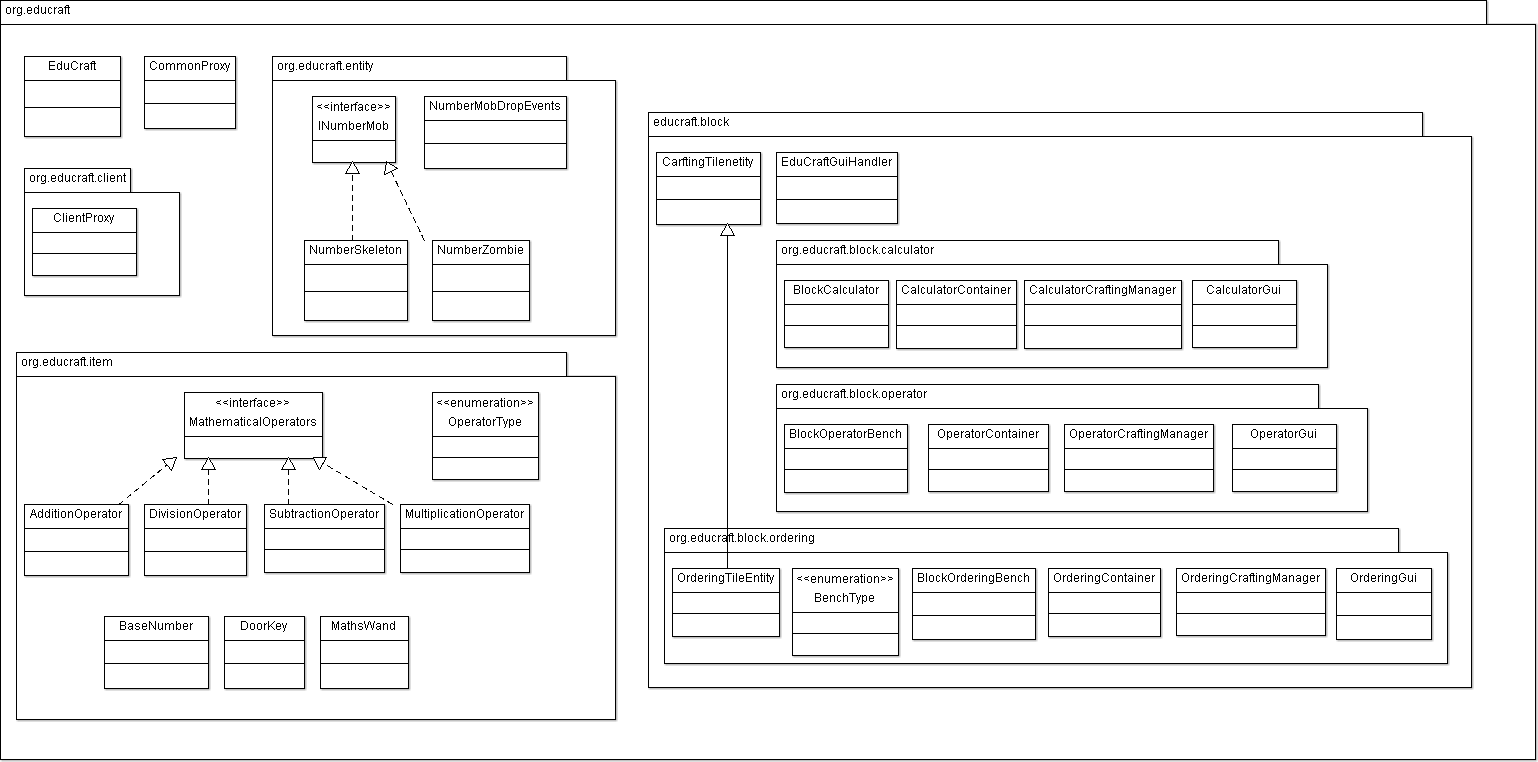
\includegraphics[width=17cm, height=11cm]{ClassDiagram}
\end{figure}

\begin{itemize}
\item \textbf{Base Mod Class}\footnote{``The base class is the class that Forge loads. All the classes in our mod have to be registered through this central location for the mod. It is advised to name this class after the name of the Mod. In our case it is EduCraft''\cite{website:forge-basemods}}\newline
The Base Mod needs to contain the following line:
\begin{lstlisting}
@SidedProxy(clientSide="tutorial.generic.client.ClientProxy",serverSide="tutorial.generic.CommonProxy")
public static CommonProxy proxy;
\end{lstlisting}

\item \textbf{Proxy Classes}\footnote{``Minecraft uses a client and server setup even on single player. The server side does all the maintaining of the world’s state while the client render’s the world. All code runs on both sides unless specified otherwise.\newline
The annotation \texttt{@SidedProxy} is used when we want the server to call the constructor of one class and the client the other. We use the proxy for registering images and hosting our GUI handler.'' \cite{website:forge-proxy}}
\end{itemize}

\section{Implementation of Constraints}
This section explains how we implemented the concept of the room and how we forced collaboration through level constraints. All levels used blocks, such as the Stone Brick block, which can not be broken with fists or an axe. This stops the player from breaking out of the level and skipping certain parts of the level without creating the correct item because we restricted the items the player could collect and create to ones which could not break through vital game blocks. We also put the game mode into adventure mode which means the player cannot take blocks from the creative tab or break any block instantly (both are possible when the player is in creative mode).

\subsection{Door Hopper Combination}
To stop players from progressing without creating the correct numbers or keys we used a door and hopper combination. We put a hopper next to the door so that when the player thinks they have the correct item they can easily throw the item into the hopper and if it is correct the door will open. By the door (as well as underneath it) there are two hoppers on top of each other and a chest next to the top hopper. The top hopper is the hopper that the player can see [Show picture]. We then add the item that we want the player to throw, into each of the five slots in the bottom hopper. We then place five redstone powder trails down, four of which will be powered, if the player throws the right item in the top hopper it will drop the item into the bottom hopper and add it to the stack. If the wrong item is thrown into the top hopper it gets pushed into the chest. This is because we can only stack identical items in the same slot therefore if all slots are taken up in the bottom hopper we can only stack those item thus forcing the player to throw the correct item.

When the correct item is thrown into the hopper the fifth powder is then powered. We can then use a repeater to boost the weak signal and place a trail of powders leading to the block below the door. The door, when powered, will open. Doors become powered when the block they sit on is powered this is why we feed the redstone powder into the block below the door and not the door itself.

\subsection{Piston Hopper Combination}
We also devised another way in which we could stop the players from progressing only when they completed the specified task. We made stacked blocks so they were two blocks high; Minecraft players can only jump one block high when in adventure mode so they would not be able to jump onto these blocks. This then means if we put these blocks in the path of the player we could force the player to complete the task. Unfortunately this leaves a problem, we needed to find a new way to push or pull one of these blocks out of the way of the player. In this instance Ian suggested the use of the stick piston block. When the sticky piston block is powered by redstone magic it would push one block outwards (positioning is key and is shown well in the image) [insert image] meaning we could push a block next two block high stack or we could pull one of the blocks away. The redstone circuits required for either of these ideas are practically the same except one has a logical not in the redstone circuit.

In reality this idea is the same as the room method using the hopper and door combination but this idea also allows us to use blocks which would fit the theme of the level. As previously mentioned keeping immersion helps the player experience and makes them feel like they’re in the game as opposed to doing mathematics in school. Moreover the piston hopper combination allows us to create more unique levels and has a lot more practical applications than the door and hopper combination. Unfortunately the door is very limited because it has to be sitting on a block and must have open spaces infront and behind it and also it can only open in two direction. The piston hopper combination does not suffer from any of these limitations.

\section{Implementation of Items}
\subsection{General Item Implementation Guide}
Most item used within the mod are from the game itself but the most important items within the game have been custom made by us. To implement a custom item is fairly simple. Firstly we extend the Item class from the original minecraft source files and then you implement the constructor which passes the itemID to the super constructor. From this point onwards anything else you implement in the constructor is optional and is totally dependant on the item you're creating. Most of the items we developed had fairly similar constructors and overridden methods.

\subsection{Number Items}
This, along with the operator item, is the most important item in the game. To implement it however is about as simple as any other item. Firstly we follow the general item implementation guide. We set the unlocalized name to number so that it is easy to use and find. Then we set its creative tab to the educraft tab so we can find it easily within the game when building levels.

When then come to the methods we have the getUnlocalizedName method which is simple terms uses the already set unlocalizedname (number) and adds a dot followed by the number that object is representing. So for example “number.35” would be the the unlocalizedName of the object representing 35. This function takes an ItemStack as its parameter this is because the actual number component of each object is encapsulated by metadata. Each item has metadata which holds the item’s damage value this can be changed for each number object so that this metadata holds is number value. We use a similar method to determine which icon each number object should have. The icon is chosen by taking the damage value and using that as the index of the icon you want in the icon array.

\subsection{Operator Items}
Once again all operators inherit from the item class. Therefore we implement the constructor in the same way as specified previously. Each construction sets the unlocalized name to a 3 letter representation of the operator plus the string “operator”. The maxStackSize is set to 4 so players can hold no more than 4 in a stack at a time. The creative tab the operators are put in is our custom educraft tab for convinience and finally we set the texture which is simply “educraft:” and the name of the operator. All operators implement the MathematicalOperator interface. The only method this interface forces is the getOperator method. This method simply returns what operator the current object is, we can use this later on in calculations because if we have two numbers and an operator object we don’t know what operator it is we just know that its some kind of operator. In addition it means we then cannot calculate the result. The method will then counteract this problem and let us know what operator that object represents. The return type of the getOperator function is actually the type ‘OperatorType’ which is an enumerated type. So for example the multiplication type is represented by the name ‘TIMES’ and contains two strings “Multiplication” and “x”. Every other operator type is represented in a similar way.

\section{Implementation of Blocks}
This section covers the most important steps that allowed us to create our own Crafting Tables with custom looks and specific behaviours.\newline\newline
During our initial attempts to create a modified Crafting Table we came across the problem of implementing our Numbers efficiently. We initially thought that we would have to hardcode every single class for each Number item that could be used in the Calculator without having to create separate recipes. This stalled our progress for while, but luckily after a substantial amount of research we found a solution. This workaround allowed us to have one BaseNumber class and every time a new BaseNumber object is created a random metadata is assigned to that specific item. The metadata defines the value, the texture used and the onscreen text displayed for that Number item. After this issue was resolved we were able to proceed with the implementation of the Calculator.\newline\newline
Minecraft distinguishes between two different ways of handling information due to being a multiplayer game, we will refer to these as Server Side and Client Side. The original Crafting Table only opens on the Client Side, which limits the interaction with this object to one player at a time. Initially we started with an implementation that only added custom looks and behaviours to our Crafting Tables. Later on, we recognised the importance of making the Crafting Tables Server Side to allow multiple players to interact with the same block simultaneously. This helped us to create an even more collaborative gaming experience.

\subsection{Extended Block Types}
The Ordering Table has three different types depending on the parity of the input numbers accepted by it. We have created an enum type named BenchType to describe the different types of Ordering Tables. OrderingTileEntity classes are created with an additional field differentiating the specific Ordering Table in the world when the block is created. This attribute will determine the behaviour of the Ordering Tables based on their type.

\subsection{CraftingTileEntity}
We created this class subsequent to our findings relating to the use of the Chest by multiple players simultaneously. We investigated how the Chest worked and found that Tile Entities are used to implement this feature.\newline
Tile Entities are bound to specific coordinates in the world and their fields hold unique values. In the case of the Crafting Table, they hold the inventory of a Block. This allows interaction that can be seen by everyone over the network.\newline
An additional field in our version of the Tile Entities keeps track of the number of players using the Block.\newline
The default constructor is not capable of setting up a crafting matrix (collection of input slots) as the CraftingTileEntity does not have a reference to a container on creation. Our work around was to initialise the CraftingTileEntity as soon as we create a container for a Block.\newline
\begin{lstlisting}
public synchronized CraftingTileEntity initialise(Container container) {
	if (this.container == null) {
		this.container = container;
this.craftMatrix = new InventoryCrafting(this.container, 1, 3);
		this.craftResult = new InventoryCraftResult();
	}
	incrUsers();
	return this;
}
\end{lstlisting}

\subsection{GuiHandler}
This class is essential for handling our custom-made GUIs. It implements the core IGuiHandler interface and has two methods:
\begin{itemize}
\item getServerGuiElement(...)\newline
generates a container, which forms the Server Side of The GUI
\item getClientGuiElement(...)\newline
generates the GUI itself, which is displayed in the Client Side
\end{itemize}

\subsection[Container]{Container\footnote{``The container is what connects the inventories of the player and tileentity to the GUI. The constructor defines the position on-screen and contents of each slot.''\cite{website:forge-container}}}
The following are the changes we made to our extended version of the container to create a custom layout of the slot matrix:
\begin{itemize}

\item in the case of a Client Side only Crafting Table, field in class:
\begin{lstlisting}
public InventoryCrafting craftMatrix = new InventoryCrafting(this, x, y);
\end{lstlisting}

\item in the case of a Server Side Crafting Table, in constructor:
\begin{lstlisting}
this.tileEntity = tileEntity.initialise(this, x, y);
\end{lstlisting}

\let\thefootnote\relax\footnote{x = the number of rows}
\let\thefootnote\relax\footnote{y = the number of columns}

\item in any case, in constructor:
\begin{lstlisting}
// adds output slot to the container
this.addSlotToContainer(new SlotCrafting(inventory.player,	this.craftMatrix, this.craftResult, 0, 124, 35));

	// adds input slots to the container
	for (int l = 0; l < x; ++l) {
		for (int i1 = 0; i1 < y; ++i1) {
			this.addSlotToContainer(new Slot(this.craftMatrix, i1 + l * 3, 30 + i1 * 18, 17 + l * 18));
		}
	}
\end{lstlisting}

\let\thefootnote\relax\footnote{x = the number of rows}
\let\thefootnote\relax\footnote{y = the number of columns}
\let\thefootnote\relax\footnote{Please note that in Slot(..., x, y, z) and SlotCrafting(..., x, y, z) the last three arguments passed in are slotIndex, xDisplayPosition and yDisplayPosition in this order. Coordinates are represented in pixels. The default size of a slot is 18x18 pixels.}

\item in the case of a Server Side Crafting Table, in the onContainerClosed() method:
\begin{lstlisting}
/**
 * Called whenever the container is closed. If no one is using the container
 * any more, then it should drop everything inside it, like a crafting
 * table.
 *
 * @param player
 *            the player who closed the container
 */
@Override
public void onContainerClosed(EntityPlayer player) {
	super.onContainerClosed(player);
	this.tileEntity.decrUsers();

	if (!this.worldObj.isRemote && !this.tileEntity.isBeingUsed()) {
			for (int i = 0; i < 3; ++i) {
				ItemStack itemstack = this.craftMatrix.getStackInSlotOnClosing(i);

				if (itemstack != null) {
					player.dropPlayerItem(itemstack;
				}
			}
	}
}
\end{lstlisting}
\end{itemize}

\subsection{Gui}
This class is responsible for the creation and display of GUIs.
There are two methods within this class. One is responsible for drawing the background and the other one is for drawing the foreground.

\begin{lstlisting}
/**
* Standard prefix for every GUI texture created for the mod.
*/
public static final String GuiTexturePrefix = "educraft" + ":" + "textures/gui/";

private ResourceLocation calculator = new ResourceLocation(EduCraft.GuiTexturePrefix+ "FileName.png");
\end{lstlisting}

\subsection{CraftingManager}
In the Crafting Manager classes for the Calculator and Ordering Bench we simplified the operation of the core version of this class. This was possible as we are not using any Recipes for implementing the logic of how the inputs are checked and the way the output is generated. Both Crafting Tables have only 3 input slots and this allowed us to validate inputs in a simpler manner.

The logic implemented for the Calculator is to have two operands (instance of BaseNumber) in slots 1 and 3 and an operator (instance of MathematicalOperator) in slot 2 of the input matrix\footnote{See Figure \ref{fig:ssot-calculator}.}.
If this condition is not met then there is nothing to generate or else it gets the metadata value (itemDamage) of the operands and the mod internally performs a mathematical operation depending on the type of operator. An output BaseNumber is generated, with the result of the operation stored in the new items metadata. There are a few cases where there is nothing generated even though the operation would be mathematically correct, but our mod does not cover the use of negative numbers, fractions and decimals. We would like to implement these concepts in future versions of the extension.

\begin{figure}[H]
\label{fig:ssot-calculator}
\caption{Screenshot of the Calculator's crafting matrix in use}
\centering
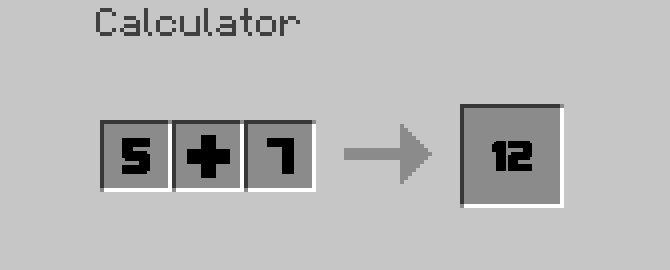
\includegraphics[scale=0.4]{calculator_use_top}
\end{figure}

The Crafting Manager for the Ordering Bench works in a similar way, but it first tests if all the inputs are numbers and then it checks if the order and the parity of the numbers are valid depending on the type of the Ordering Table.
Finally it generates a coloured key, with the colour depending on whether the bench was set to accept odd numbers,
even numbers, or all numbers\footnote{See Figure \ref{fig:ssot-ordering}.}.

\begin{figure}[H]
\label{fig:ssot-ordering}
\caption{Screenshot of the Ordering Bench's crafting matrix in use}
\centering
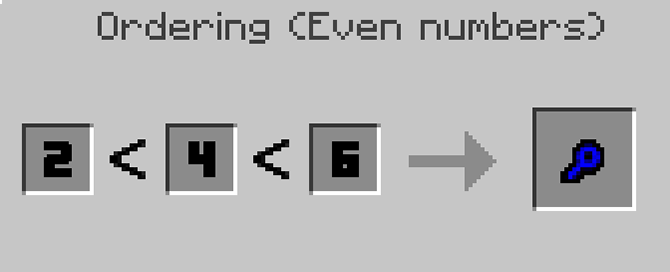
\includegraphics[scale=0.4]{ordering_use_top}
\end{figure}

We decided to keep the way the core Crafting Manager works for the Operator Bench. This bench has the same behaviour as the core Crafting Table. The only modifications are the visuals and the recipes accepted. We wanted to limit the items that could be crafted by the players in the mod. We achieved this by placing only our own modified versions of the Crafting Tables in our levels. These benches accept only our custom recipes which we defined for the crafting \footnote{``Crafting is the method by which many blocks, tools, and materials are made in Minecraft. In order to craft something, players must move items from their inventory to a crafting grid. A 2×2 crafting grid can be accessed from the player's inventory. A 3×3 grid can be accessed by right-clicking a Crafting Table.''} of the mathematical operators\footnote{See Figure \ref{fig:ssot-operators}.}.
All these recipes are ShapedRecipes\footnote{``Shaped recipes come in all sizes from 1x1 to 3x3. Strings are used for the recipe shape and values.''\cite{website:forge-shaped}} used in the original version of Minecraft.

\begin{figure}[H]
\label{fig:ssot-operators}
\caption{Screenshot of the Operator Bench's crafting matrix in use}
\centering
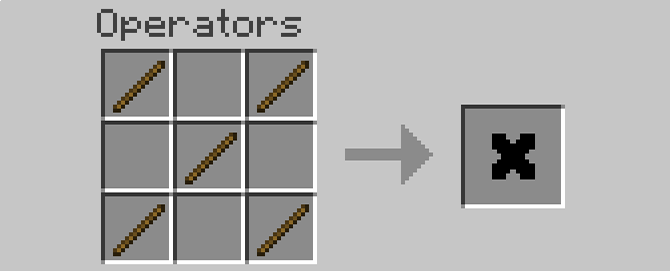
\includegraphics[scale=0.4]{operator_use_top}
\end{figure}

The method signature is roughly as follows:
\begin{lstlisting}
this.addRecipe(String row1, [String row2[, String row3]]
        char itemType1, ItemStack itemStackType1[, ... char itemTypeN, ItemStack itemStackTypeN]);
\end{lstlisting}
A list of all the recipes added to the Operator Bench:
\begin{lstlisting}
/** A list of all the recipes added */
private List<IRecipe> recipes = new ArrayList<IRecipe>();

private OperatorCraftingManager() {
	ItemStack sticks = new ItemStack(Item.stick);
	this.addRecipe(new ItemStack(EduCraft.ADD_OPR), " s ", "sss", " s ", 's', sticks);
	this.addRecipe(new ItemStack(EduCraft.SUB_OPR), "   ", "sss", "   ", 's', sticks);		this.addRecipe(new ItemStack(EduCraft.MUL_OPR), "s s", " s ", "s s", 's', sticks);
	this.addRecipe(new ItemStack(EduCraft.DIV_OPR), "  s", " s ", "s  ",'s', sticks);
}
\end{lstlisting}

\section{Implementation of Mobs}
\subsection{General Mob Implementation Guide}
All monsters(mobs) in the game are entities. Each monster we implemented was therefore also an entity and since we decided to use well known minecraft monsters the zombie and the skeleton it was natural we would just inherit from these two already existent classes. When implementing a mob there are a few simple steps. Firstly the constructor, the constructor should pass the world to the super constructor. The world should be passed into the constructor as a parameter. You can then set what item for the mob to drop by using the this keyword followed by ‘droppedItemId’ and make it equal to the ID of the item you wish the mob to drop. You can then set the name of the monster which is seen by the player in game by using the method setCustomNameTag and then giving it a string.

Each monster class has many methods which help with setting which will drop. In many classes such as the skeleton class it does not use the normal method of dropping a default item. It uses the ‘dropFewItems’ method so a skeleton will always drop multiple items, it may also drop a rare item through the dropRareDrop item this has a significantly lower chance. Most monsters have the rare drop method and use it, our custom monsters only implement the getDropItemId so that we can get what item the monster will drop. Not only do we not implement the other drop methods we override them and leave them empty. If they’re not overridden and left empty the monster may begin to drop other items such as helmets and bows because the minecraft engine has a chance to randomly invoke the rare drop or the case of the skeleton it will always invoke the multiple item drop method. These methods will of course be those from the superclass.

\subsection{Discussion Of Mob Drops Event}
The ‘numberMobDropsEvent’ is a class which handles the dropping of number items from all custom monsters in the game. When a monster dies it calls the ‘onEntityDrop’ method which has the event has a parameter. We can use this parameter to get what the monster was killed by, if we check this and it turns out to be the maths wand then we make sure we drop the number item and not some other item. This method also does one more thing it checks what monster actually died so if it was a skeleton number zombie the random number generated will be a multiple of ten if it was a number zombie it will be a number between 1 and 10 inclusive. If any other monster died the handler will do nothing and it will reach the end of the method.

\section{Implementation of Locations}
We used creative mode\footnote{``Creative mode is one of the main game modes in Minecraft. This mode strips away the survival aspects of Minecraft and allows players to easily create and destroy structures. Creative mode allows players to destroy all blocks instantly (including normally-indestructible blocks such as bedrock) and the ability to fly. Players are given an infinite number of blocks to build with and no health or hunger bar thus rendering the player immune to all damage.''\cite{website:minecraft-creative}} in Minecraft to create all the different locations (levels) in our world. In order to make the visual experience in the mod more enjoyable we used a world editing tool called MCEdit to create a small forest and mountains in the surrounding area of the locations.

We have also created our own tab for easier access of custom elements in the inventory list. We added the following line to the constructors of all elements created by us:
\begin{lstlisting}
setCreativeTab(EduCraft.tabEduCraft);
\end{lstlisting}
\begin{figure}[h!]
\centering
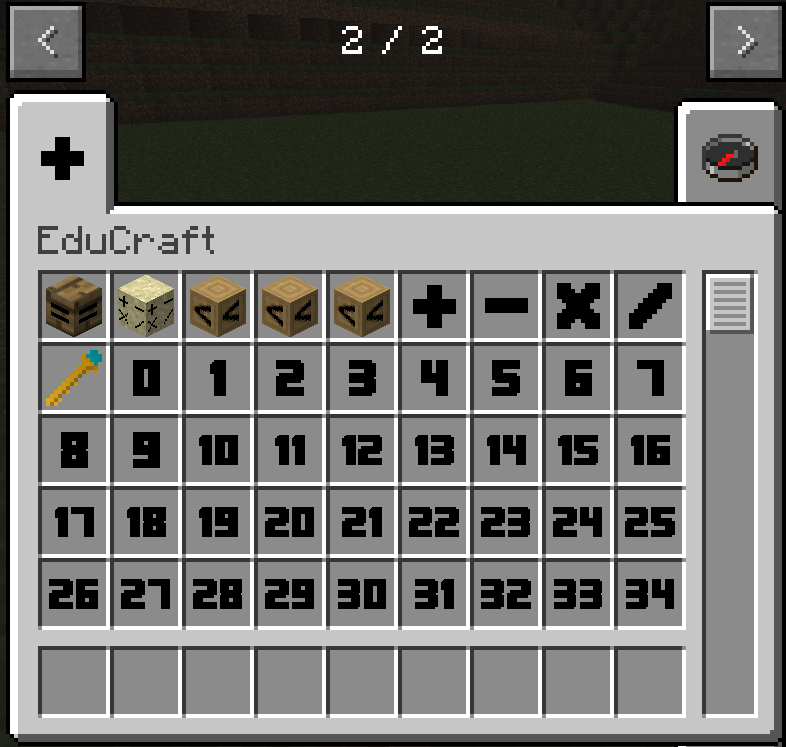
\includegraphics[scale=0.4]{educraft_tab}
\caption{"Screenshot of EduCraft custom tab in game inventory"}
\end{figure}

\subsection{Castle}
The collaborative element of this level was implemented by setting a task to create four different operators, which would open doors to four different rooms using the hopper system in the first part of the level. Each room has a key inside and all four keys are needed to allow the players to progress to the next part of this level.

In the next part each player will have to pick up a Maths Wand and kill some Zombies and collect enough numbers to be able to use the Ordering Bench. A correct ordering of numbers will generate a key that opens the door leading to the final part of this level.

In the final part the team has to obtain a specific number through a series of mathematical operations to be able to leave the level through the exit. There is a chest full of Mathematical Operators which they can use within the Calculator. The team has to kill Zombies and Skeletons to collect the numbers dropped by the monsters.

All tasks in this part are designed so no one can progress without the help of the others. This was set to be a tutorial level which would allow the players to familiarise themselves with the game play of the mod.

\subsection{Pyramid}
This level forces the team to split up at the beginning. This is achieved by only allowing two players inside the Pyramid;
as soon as there are two players inside the entrance is blocked. A plan of this level's design is shown in
Figure \ref{fig:pyramid-layout}.

The interior of the Pyramid has two floors and it is divided into four sections. The Pyramid is surrounded by a garden with fences and walls so as to prevent the outside team from wandering around in the world. Each inner section has its own corresponding outer garden section. Neither the inside nor the outside team can go to the next section without collaboratively working towards a goal set for each section of the level.

There is an exit through the top of the Pyramid for the inside team. The inside team can only leave once each subteam has generated a key in the fourth section of the level. The outside team can climb the stairs on the side of the Pyramid in the fourth section and throw their key inside for the other team. The inside team should have two keys by this point and each key will move a block, creating a path to leave. Once all the players are reunited, they can leave through the level exit, which located in the final garden section.

In each section the resources available are limited for each subteam, for example in one section the inside team has access to sticks and an Operator Bench, but not to any numbers. In the same section the outside team has the opportunity to kill Zombies or Skeletons to be able to collect numbers and they also have a Calculator to generate numbers.

We implemented a system that allows the teams to send items back and forth in minecarts that move on rails. This will force them to communicate their requirements to each other.

\begin{figure}[h!]
\label{fig:pyramid-layout}
\caption{Sketch of the Pyramid's layout}
\centering
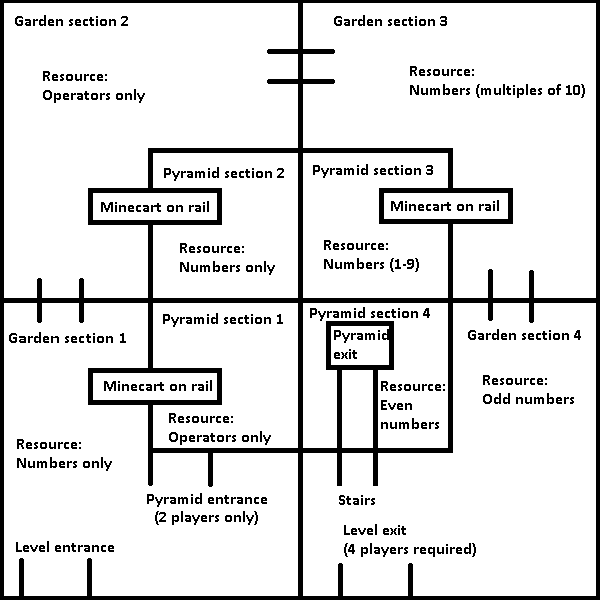
\includegraphics[scale=0.65]{pyramid}
\end{figure}

\subsection{Rook}
The Rook has two floors and on each floor there are two rooms. Only the first two players to arrive can enter each room. The subteams’ resources are limited in a similar manner to the Pyramid. The rooms on the same floors share a wall. In each of these walls there is a Calculator built-in, which can be used by the subteams to pass items to each other and to execute some mathematical operations together.

In order to leave the rooms the teams must generate a specific number and throw that number in the hopper by the exit. Each exit is connected to a staircase that leads to the floor above. The “roof top” of the Rook is the final destination in our game. It is relatively elevated, so the players can have a look around and see the world and all the levels they have completed.

\chapter{Testing and Analysis}

This chapter describes the field testing the project underwent,
along with a discussion of the results obtained.

\section{Pilot test}
This section describes the testing we carried out with Ed (need to
change his name), and the lessons we learnt.

\section{Firbeck Academy}
This section describes the day of testing in Firbeck Academy, with
some brief observations on what we saw.

\section{Discussion}
This section then explores the results we obtained, draws conclusions,
and explores directions for further development of the project.

\chapter{Reflections}
\label{ch:reflections}
Reflection is a very important part of a successful project. Looking back on a process you 
have gone through and considering what went well, what did not and what could have been 
done differently is a very worthwhile experience as it gives you the wisdom to improve 
yourself and your work in the future. Done well, reflection can give an objective evaluation of the success of a project which is unmistakably important.\newline

Communication and group work was generally very good, although by no means perfect. We 
used online resources and websites to communicate and coordinate work, which was useful 
for keeping everyone up to date outside of our face-to-face meetings. We held formal 
meetings most weeks with our supervisor, Peter Blanchfield, in order to discuss progress, 
goals, obstacles, and to get advice on various aspects of the project. These were 
supplemented by informal meetings with the group alone, which helped team coordination 
and setting out a plan. The importance of these meetings cannot be overstated, as they 
were what kept the ball rolling throughout, and ensured decisions were made, work got done 
in time and documentation of this all was kept so as to have a permanent record to refer to 
at all stages of the project. As such, these meetings were very useful, although did underline issues we had with group work; this was due to lack of involvement and communication by some members of the group at certain stages of the project. If group dynamics had been better, then we could have achieved more – for example we had plans for an iOS app that never came to fruition due to lack of time. Furthermore, we could have implemented more mathematical concepts to challenge older players for whom the puzzles and concepts covered in our current mod are trivial. Just as importantly were issues we had with players abusing the environment and playing the game in a non-productive way, which required level design decisions to minimise. With better group dynamics and more collective time, we could have dealt with the problems faced a lot sooner, allowing us to implement more of the desired features and meet more of the initial requirements we set.\newline

Progress on the mod was sometimes slowed down by technical issues, for example in our 
implementation of custom Minecraft items and blocks such as the numbers and the 
Calculator Bench. However, we dealt with these obstacles well, because when our initial 
ideas did not work or were implemented in a flawed manner, we would take a step back and 
research the problem and consider available technology and tools in order to look for 
workarounds. Using git for version control was crucial as we could try out some code, and if it did not solve our issue or had unexpected consequences then we could simply roll back to a previous version and start research and work on a new or modified solution. Pairs 
programming was also an extremely helpful method for coding, using the combined 
knowledge of two people made writing competent, useful and functional code that much 
easier, and was immensely important in dealing with bugs, and tackling obstacles of 
implementation. All things considered, our approach to technical issues and the process of 
searching for a solution was difficult and time-consuming, but ultimately worth it as we often developed simple, clever and effective solutions.\newline

Overall, the project was largely a success. Despite limitations and issues faced, we have 
created a playable mod that fulfils the expectations of our original project description: ``The project would aim at developing mods for the Minecraft game in which players could only win by collaborating with others''. Testing the game ourselves, with individual children and as well at the school showed promise that collaborative learning in Minecraft is possible, even though there were a lot of problems and shortcomings, as outlined in the Testing and Analysis section of this report. Most of the people involved enjoyed the process and were excited about the project's potential, and we believe that EduCraft demonstrates the usefulness Minecraft can have as an educational tool for collaborative learning, and are looking forward to further development.


\appendix
\chapter{Class Diagram}
\label{apdx:class-diagram}

\begin{landscape}
\begin{figure}[H]
\label{fig:class-diagram}
\caption{UML class diagram of EduCraft}
\centering
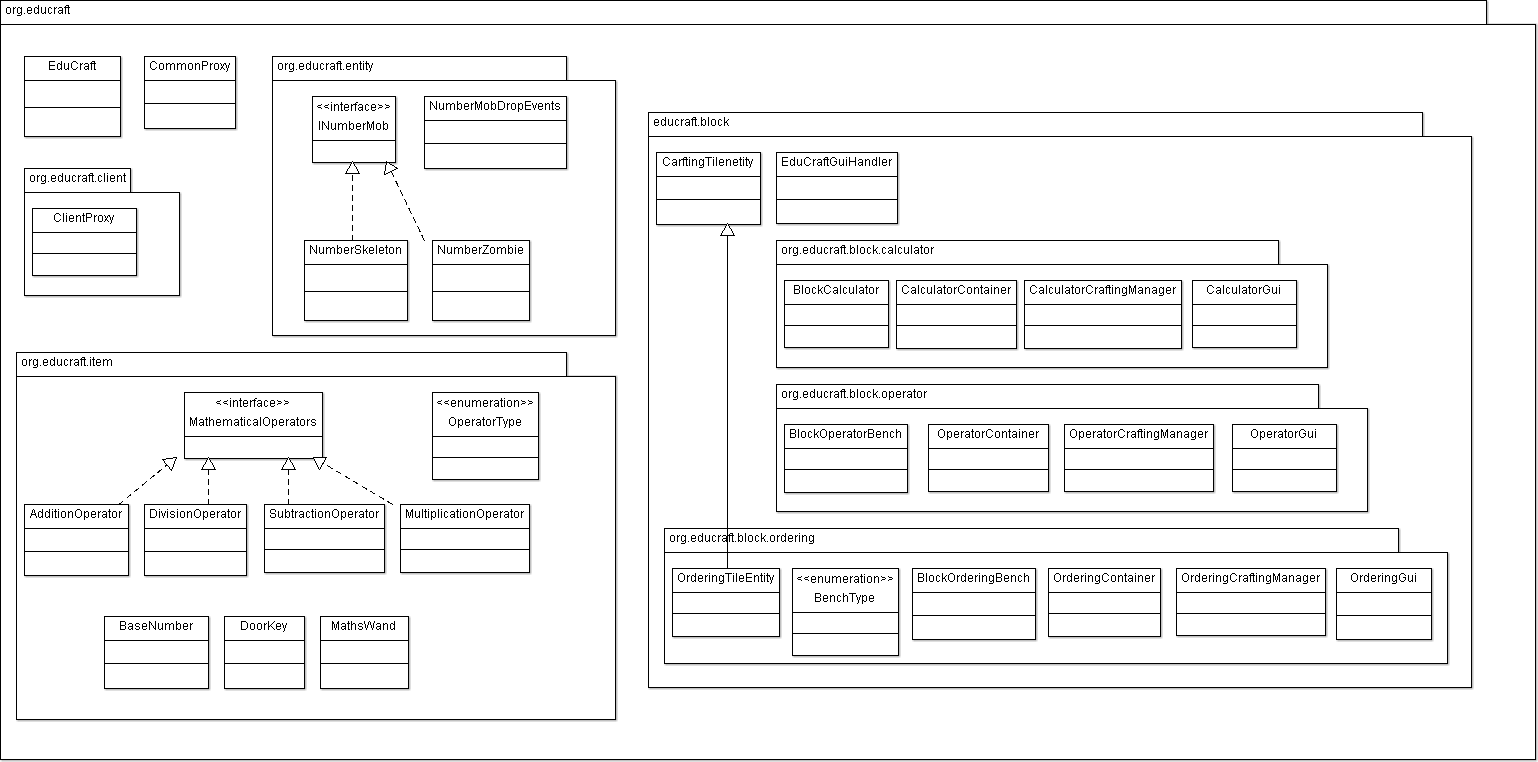
\includegraphics[width=21cm, height=15cm]{ClassDiagram}
\end{figure}
\end{landscape}

\chapter{Unit Testing}
\label{apdx:unit-tests}

\section{Approach}
Unit testing is considered a vital part of any software engineering
project, as it allows the team to assert that the individual components
of the system function as intended \cite{sommerville11}. They also
provide a convenient means of carrying out regression testing: when
changes are made, the same tests can be re-run, theoretically with the
same outcome.

From the outset, the EduCraft developers were concerned with how to
effectively test the mod, particularly key elements of it such as the
calculator block.

\section{JUnit and Minecraft Forge}
JUnit is a simple unit testing framework for the Java language \cite{website:junit},
and as the Eclipse IDE has built-in support for JUnit, it was the first choice
of testing tools to use.

However, on beginning to write unit tests for the mod, we encountered
a number of problems. A number of the classes comprising the core of
the Minecraft game cannot be instantiated unless there is an underlying
game client running, and this includes several key classes used in
our mod\footnote{\texttt{net.minecraft.item.ItemStack} is a prime
example.}.

This limitation meant that very few meaningful test cases could be written,
since the tests requiring these uninstantiable classes would not
compile. It was the view of the developers that, although unit testing is
considered to be best practice in software engineering \cite{sommerville11},
an alternative testing strategy would have to be devised for the project.

\section{In-Game Testing}
The approach decided upon was to set up a very basic `Test World'
with no terrain and no entities apart from the player. New blocks would
be placed in this world, and their functionality tested in-game.
Although such an approach means that testing documentation is
not available, the entire development team agreed that this was the
best solution available, given the limitations of the API.

\chapter{Game measures}
\label{apdx:measures}
These measures were developed based on the PhD thesis of Nicola Whitton \cite{whitton07}.
They were designed not to be used as interview questions, but instead as prompts to
the testers, to help them focus their observations on key things.

The use of these measures is described in Chapter \ref{ch:testing}.

\section{Engagement with the game}

\begin{enumerate}
\item Measure average time it takes for a group of players to complete a level

\item Ask general questions about how challenging and immersive the game was
\begin{enumerate}
    \item Were there any points where they were confused or not sure what was going on?
    \item Were there aspects of the game that were too easy or too hard?
    \item How did the difficulty of the game change as you progressed through levels
\end{enumerate}

\item How much of game time is spent on task?
\begin{enumerate}
    \item What possible distractions are there?
\end{enumerate}

\item How often do they ask for help understanding the game concept?
\begin{enumerate}
    \item What sort of questions did they ask?
\end{enumerate}

\item Did they like the zombie characters?

\item What were their thoughts on the level maps?
\begin{enumerate}
    \item Were they interesting and varied?
\end{enumerate}

\end{enumerate}

\section{Use of collaboration}
\begin{enumerate}

\item How well did they communicate?

\item Did they understand the need to collaborate in order to advance?

\item Did they use their maths skills or did they randomly guess and match operators?

\end{enumerate}

\section{System integrity}
\begin{enumerate}

\item Did the game crash?

\begin{enumerate}
    \item What was the reason?
\end{enumerate}

\end{enumerate}

\chapter{User Guide}
\label{apdx:user-guide}

This appendix presents a brief guide to using EduCraft. More extensive
documentation, including videos, is available at \texttt{TosinAF.github.io/EduCraft}.
URLs to the relevant videos are included in the sections below.

\section{Controls}
EduCraft uses the same controls and follows the same basic principles of regular Minecraft,
and so anyone with a basic understanding of Minecraft should be able to play Educraft. Even
without experience, the controls and concepts can be picked up quickly, and the main level
design we have produced incorporates a tutorial section at the start.

A full description of Minecraft's default controls is available on the official
Wiki page \cite{website:minecraft-controls}.


\section{Tutorial walkthrough}
This section provides a summary walkthrough of the first level of the game,
which is used as an introduction to EduCraft's new mechanics.

\subsection{First room}
The first step in the tutorial is to collect logs, which can be turned into planks and
then sticks for crafting purposes\footnote{Turning logs into sticks: \texttt{www.youtube.com/watch?v=Q3aMJ5jwxuM}}.
Sticks are important as they are what the player needs to craft operators. This is done by creating
the pattern of the desired operator in the Operator Bench, which can be used in a similar
way to a crafting table in regular Minecraft.
Players need to make patterns +, -, /, or X for plus, minus, divide, and times
\footnote{Creating operators: \texttt{www.youtube.com/watch?v=Mrg\_mkqP-D8}}.
The final step is to unlock doors by throwing the appropriate operator into the hopper
for the adjacent door\footnote{Throwing items into hoppers: \texttt{www.youtube.com/watch?v=0a-KPj\_FB80}},
and then throwing the keys found inside into
the hoppers at the end of the corridor.

\subsection{Second room}
The second room introduces players to the concept of killing enemy characters
in order to collect numbers\footnote{Killing monsters: \texttt{https://www.youtube.com/watch?v=ZswqlwMR3f4}}.
The second room requires the player to collect three numbers and then place them in
an Ordering Bench, in order to obtain a key to unlock the second
door\footnote{Using the ordering bench: \texttt{https://www.youtube.com/watch?v=MQTVB4etTfE}}.
The ordering bench in the second room will accept all numbers; benches later in the game
will accept either odd or even numbers only.

\subsection{Third room}
The final room works in a similar fashion to the second, except that the players
must use the Calculator provided to produce a target number
\footnote{Using the calculator: \texttt{https://www.youtube.com/watch?v=uxbQ4CySm30}},
rather than using and ordering bench to gain a key.


\section{Collaboration}
Educraft requires collaboration between teams of players in order for progress to be made.
One way this is done is by the necessity for players to pass resources (operators, numbers)
to each other by using rail carts. The player places the item(s) they want to send to the other
team into the chest on the cart, and then presses the button to send the cart
\footnote{Using a minecart to exchange items: \texttt{https://www.youtube.com/watch?v=k-GD8Vr8fhc}}.


\bibliography{bibliography}

\end{document}
